% !TeX root = e4-tp2-ej2
\documentclass[e4-tp2-main.tex]{subfiles}

\begin{document}

\section{Convertidor boost para l\'ampara LED de potencia}

\subsection{Efectos de temperatura en los LEDs}

\begin{wrapfigure}[20]{L}{0.55\textwidth}
    \centering
    \begin{subfigure}[t]{0.25\textwidth}
    	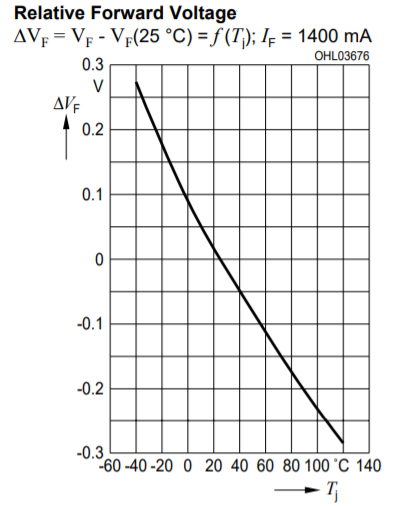
\includegraphics[width=\textwidth]{images/ej2/Cambio_Vf_LED.png}
    	\caption{Cambios en $V_f$}
    \end{subfigure}
    \begin{subfigure}[t]{0.25\textwidth}
    	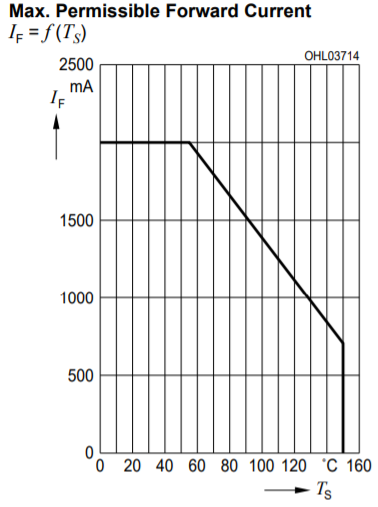
\includegraphics[width=\textwidth]{images/ej2/Cambio_If_LED.png}
    	\caption{Cambios en $I_{f_{MAX}}$}
    \end{subfigure}
    \caption{Efectos de la temperatura en los LEDs}
    \label{fig:Efec_Leds}
\end{wrapfigure}

Se utilizaron los LEDs OSRAM LUW-W5AP, los cuales a medida que aumenta su temperatura se producen variaciones de la tensión de forward ($V_f$) y la máxima corriente de forward soportada ($I_f$). Donde ante un aumento de la temperatura tenemos un aumento de $V_f$ y una disminución de $I_{f_{MAX}}$.\\

Como puede observarse de los gráficos obtenidos del datasheet en la figura \ref{fig:Efec_Leds} se puede despreciar los cambios producidos en $V_f$ debido a que los cambios de corriente son mucho más apreciables.\\

\end{document}

